\documentclass[a4paper]{article}   
\usepackage{cite} 
\usepackage{hyperref} 
\usepackage{longtable} 
\usepackage{verbatim} 
\usepackage{rotating}
\usepackage{Sweave}
\begin{document}
\Sconcordance{concordance:EHIs_transformations_doc.tex:EHIs_transformations_doc.Rnw:%
1 6 1 1 0 49 1 1 27 2 1 1 16 3 1 1 30 3 1 1 13 16 1 1 57 20 1 1 32 4 1 %
1 13 2 1 1 10 5 1 1 42 15 1 1 47 12 1 1 20 18 1 1 81 6 1 1 47 10 1 1 %
107 110 0 1 3 5 1 1 51 2 1 1 28 2 1 1 31 2 1 1 18 21 1 1 15 6 1}

\title{Extreme Heat Indices} 
\author{Ivan C. Hanigan$^{1}$}
\date{\today}                 
\maketitle
\begin{itemize}
\item [$^1$] National Centre for Epidemiology and Population Health, \\Australian National University.
\end{itemize}

\setcounter{page}{1}
\pagenumbering{roman}
\tableofcontents 
\pagenumbering{arabic}
\setcounter{page}{1}

\section{Intro}
The paper by Nairn et al proposed 3 new Extreme Heat Indices (EHIs) we were asked to investigate.  \url{http://www.cawcr.gov.au/events/modelling_workshops/workshop_2009/papers/NAIRN.pdf}.  The following description is reproduced from their paper.

 The EHIs they propose are based on average daily temperature (ADT), defined as the average of the
 maximum and minimum temperature (Tmin) within a 24-hour 9 am to 9 am (local time) day, which
 corresponds to the daily temperature observation cycle in Australia. In practice, this means that the early
 morning Tmin typically follows the afternoon Tmax in time.
 The first EHI we propose is an acclimatisation index, defined as: 
 
 $EHI{accl} = (Ti + T{i}-1 + T{i}-2)/3 - (T{i}-3 + \ldots + T{i}-32)/30$
 
 Where Ti is the ADT for day i. In other words, EHI(accl.) is the difference between the mean ADT over a three-day period and the mean ADT over the preceding thirty days. Positive values are associated with relatively hot weather, or excess heat, negative values with relatively cool weather. This index is very much a relative one, excess heat according to this index is possible in summer and winter
 alike. Also, its values are not expected to become more extreme under a general warming trend.
 
 The second EHI is more an absolute index, and is defined as:

 $EHI{sig} = (Ti + T{i}-1 + T{i}-2)/3 - T{95}$
 
 Where T95 is the 95th percentile of ADT. We use the 30-year period 1971-2000 for the calculation of T95, and the
 calculation is across all days in the year. With this second index, excess heat is typically only possible in the summer half-year, because hot winter weather isnt hot by annual standards. The comparison against T95
 gives a measure of the statistical significance of the event. Unlike EHI(accl.), this index is expected to
 become more extreme under a general warming trend, provided a fixed climatological period for T95 is
 adopted. Lastly, the excess heat factor (EHF) is defined as:
 
 $EHF = | EHI{accl} | \times EHI{sig}$
 
 which obviously implies that $sign(EHF) = sign(EHI{sig}) - EHI{accl}$ acts as an amplification term on EHI(sig.).
 
 Nairn et al also integrate the indices:  In one method they count the consecutive days in which the index is positive.
 They also sum the daily values of EHF across entire heat waves (TASK defined how?  Number of consecutive days over the threshold used in Adelaide by others?  Figures 1-4 suggest it is not the 5 over 35 or 3 over 40 as they integrate from 7 Jan to 18 Feb 2009  \url{http://www.bom.gov.au/announcements/media_releases/sa/20100115_First_Heatwave_SA_Jan.shtml}).  Only positive daily values of the EHF contribute to the integration, negative values are treated as if they were zero.  This gives a good insight into the intensity of a heatwave, however unless we define a threshold to start and stop counting we cant do this (we could use periods where the EHI is continously positive?).
 

\subsection{The R code that produced this report}
I support the philosophy of reproducible research \url{http://aje.oxfordjournals.org/content/163/9/783}, and where possible I provide data and code in the statistical software R that will allow analyses to be reproduced.  This document is prepared automatically from the associated RNW file.  If you do not have access to the RNW file please contact me.

%% \subsection{tools}


\subsection{load}
The BoM data are used as a test case \url{http://www.bom.gov.au/climate/change/hqsites/}.  Metadata are available at \url{http://www.bom.gov.au/climate/change/hqsites/about-hq-site-data.shtml#format}.
 

\subsection{qc graph}
A plot of the raw data is shwon in Figure \ref{fig:023090.png}.
 

\begin{figure}[!h]
\centering
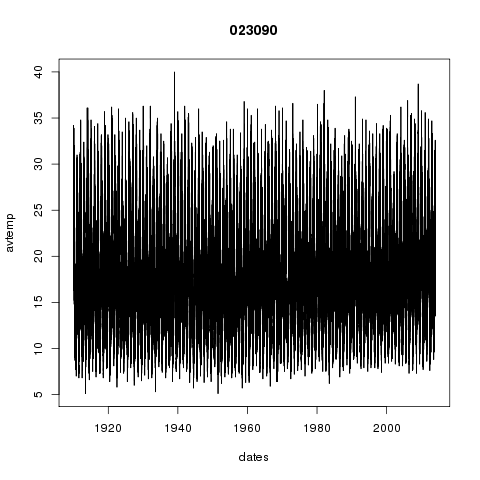
\includegraphics[width=\textwidth]{023090.png}
\caption{023090.png}
\label{fig:023090.png}
\end{figure}
\clearpage

\subsection{EHI{accl}}

 $$EHI{accl} = (T{i} + T{i-1} + T{i-2})/3 - (T{i-3} + \ldots + T{i-32})/30$$
 
 where 
 $T{i}$ is the ADT for day i. 
 In other words, $EHI{accl}$ is the difference between the mean ADT over a three-day period and the mean ADT over the preceding thirty days
 

\begin{figure}[!h]
\centering
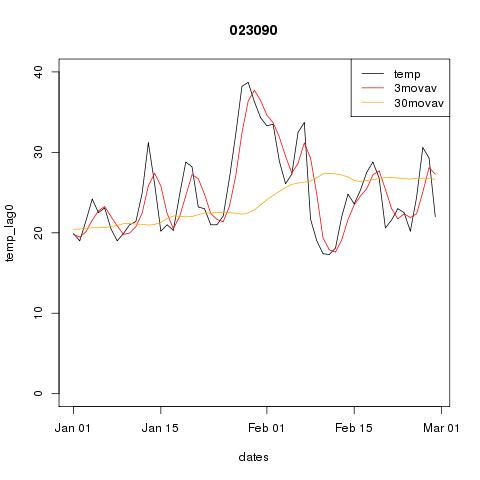
\includegraphics[width=\textwidth]{023090movavs.png}
\caption{023090movavs.png}
\label{fig:023090movavs.png}
\end{figure}
\clearpage

\subsection{EHI{sig}}
$$EHI{sig} = (Ti + T{i}-1 + T{i}-2)/3 - T{95}$$

 where T{95} is the 95th percentile of ADT. 
 
 Nairn et al use the 30-year period 1971-2000 for the calculation of T{95}, and the calculation is across all days in the year.  
 
 TASK the index is expected to become more extreme under a general warming trend, provided a fixed climatological period for T{95} is adopted.  Is this a good thing or not for heat wave research?
 We decided to use the entire study period in our first cut because we only run from 1997 to 2007 and this is a bit limited in terms of any reference period.
 The algorithm will include an option to set the reference period or take all data available.
 
 

\subsection{EHFS}

 $$EHF = | EHIaccl | \times EHI{sig}$$
 

\section{Check the results}


\subsection{summary}

Figure \ref{fig:Figure1.png} shows station-based results for Adelaide in January and February 2009. The station-based data are obtained using the Adelaide (Kent Town) site (023090), (NOTE not imputed, Nairn et al supplemented their data using Adelaide (West Terrace) site (023000) data in the early part of the base period 1971-2000, we will access information from neighbourhing stations via our spatial interpolation methods).
 The topleft plot shows daily average temperature data, the topright plot shows the EHI{accl} and EHI{sig} values while the bottomleft plot shows the EHF (all values are plotted against the last day of the integrated calculation period).
 

\begin{figure}[!h]
\centering
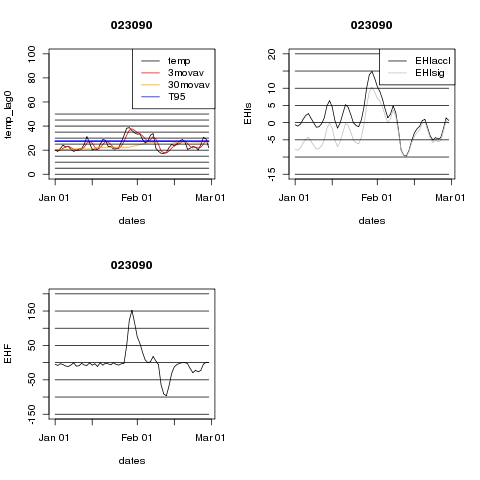
\includegraphics[width=\textwidth]{Figure1.png}
\caption{Figure1.png}
\label{fig:Figure1.png}
\end{figure}
\clearpage

\subsection{Ask BoM what they think is a good threshold}

We asked Richard Broome to ask BoM about a threshold.  He reported: It seems they are planning to call any day with an EHF >1 a heat wave. Because these days happen pretty frequently, they also plan to have an ``extreme heat wave".  This is yet to be defined, but they made one suggestion, which was to call an extreme heat wave any day with an EHF greater than the highest 20\% of EHF based on historical data (does that make sense?). However, they seemed very open to suggestion and keen to get health input.
 
 So lets have a look at what that would mean for the exemplar dataset from Adelaide.  In Figure \ref{fig:checkEHFagainstQuantiles.png}  the percentiles of EHF are shown.  The top left plot shows the EHF against the percentile ranks of average daily temperature during the 1970-2000 period.  The top right plot shows the heatwave threshold at EHF of 1 against the percentiles of ADT and implies that 75 percent of EHF heatwaves are captured by the 95 percentile of daily temperature. The bottom left plot is just the raw daily temps against EHF and the bottom right is the EHF heatwaves ranked as percentiles, and the suggested upper quintile threshold identified (30.1 EHF).
 
 

\begin{figure}[!h]
\centering
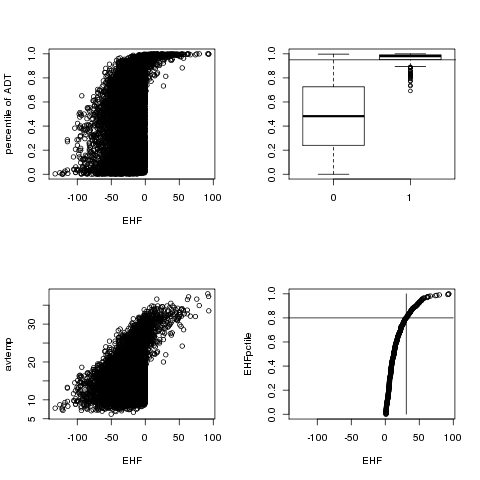
\includegraphics[width=\textwidth]{checkEHFagainstQuantiles.png}
\caption{checkEHFagainstQuantiles.png}
\label{fig:checkEHFagainstQuantiles.png}
\end{figure}
\clearpage

\subsection{How would the Adelaide heatwave look}

The exemplar heatwave that Nairn et al use in their document is shown again in Figure \ref{fig:Figure1withHeatwaves.png} with the addition of the proposed heatwave thresholds.  It can be seen here that the threshold of 1 is very close to the 95th percentile, and that the extreme heatwave threshold gives a more conservative estimate of the heatwave duration.
 

\begin{figure}[!h]
\centering
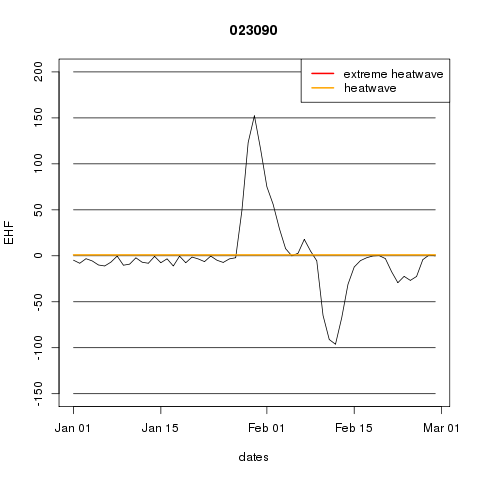
\includegraphics[width=\textwidth]{Figure1withHeatwaves.png}
\caption{Figure1withHeatwaves.png}
\label{fig:Figure1withHeatwaves.png}
\end{figure}
\clearpage

\subsection{Propose a threshold method based on Hutchinson}

I propose we follow the drought index method of Professor Mike Hutchinson described in Smith D, Hutchinson M, McArthur R. Climatic and Agricultural Drought: Payments and Policy. Canberra, ACT: Centre for Resource and Environmental Studies, Australian National University. 1992.  
 
 That method integrates consecutive months of lower than average rainfall (based on percentiles of 6-monthly running totals of the rainfall records at each location).  The integrated score is constructed either by counting months or summing the inverted percentile value.  A drought is then declared when the integrated score goes beyond a threshold (calibrated to the NSW government drought declarations).  
 
 I propose we count the number of days that EHIaccl and EHIsig are consecutively positive, and sum the integrated EHF score.  Then we calibrate the threshold at which a heat wave is declared to some well-known heatwaves such as the two Adelaide heatwaves shown in Nairns paper, the 2006 new years day heatwave on the south coast of NSW and the November 2009 heatwave in Adelaide \url{http://bravenewclimate.com/2009/11/14/three-record-heatwaves-seaust/}.
 
 We could perhaps use the Adelaide definition of 5 consecutive days above 35?  Although the bom site does state that This definition is only applicable to Adelaide since climatic norms differ across the state. 
 

\subsection{Add this to the summary}

Figure \ref{fig:thresholds.png} shows this proposed threshold definition applied to the 2009 Adelaide heatwave.
 
 This shows that counting the days where the acclimatisation (EHIacclCount) method is used there are more days classed as heatwave than when the 95th percentile is used (EHIsigCount).  The integration of the EHF shows that the heatwave was really entirely defined by the days between 28 Jan and 8 Feb 2009.
 

\begin{figure}[!h]
\centering
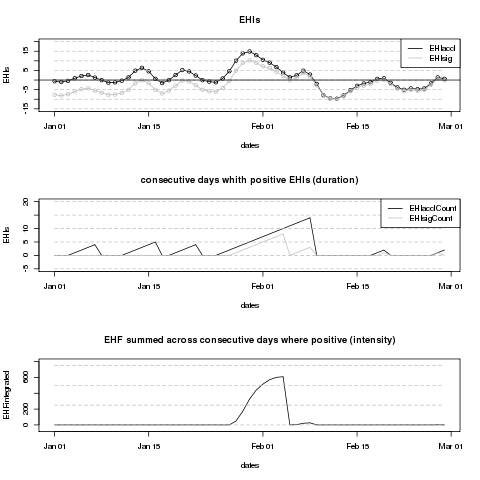
\includegraphics[width=\textwidth]{thresholds.png}
\caption{thresholds.png}
\label{fig:thresholds.png}
\end{figure}
\clearpage

\subsection{Make an R function to do the work}

\begin{Schunk}
\begin{Sinput}
> ######################
> #tools,  Make an R function to do the work
> ######################
>       
> 
>  
>  EHIs <- function(analyte = data_subset,
+   exposurename = 'air_temperature_in_degrees_c_max_climatezone_av',
+   datename = 'date',
+   referencePeriodStart = as.Date('1971-1-1'),
+   referencePeriodEnd = as.Date('2000-12-31'),
+   nlags = 32) {
+   # TASK SHOULD WE IMPUTE MISSING DAYS?
+  
+   # first get lags
+   # TASK THERE IS PROBABLY A VECTORISED VERSION THAT IS QUICKER?
+   # TASK it is rollmean from the zoo package
+   # ALTHOUGH THAT DOESNT HANDLE NAs SO TRY ROLLAPPLY?
+   analyte$temp_lag0 <- analyte[,exposurename]
+   exposuresList <- 'temp_lag0'
+   # make sure in order
+   analyte <- arrange(analyte,  analyte[,datename])
+   # lag0 is not needed
+   for(lagi in 1:nlags){
+  	# lagi <- 1
+  	exposuresList <- c(exposuresList, gsub('lag0',paste('lag', lagi,sep=''), exposuresList[1]))
+  	analyte[,(ncol(analyte)+1)] <- Lag(analyte[,exposuresList[1]],lagi)
+  	}
+   exposuresList <- exposuresList[-1]
+   names(analyte) <- c(names(analyte[,1:(ncol(analyte)-nlags)]),exposuresList)
+   # head(analyte)
+   # now 3 day av
+   analyte$temp_movav <- rowMeans(analyte[,c('temp_lag0','temp_lag1','temp_lag2')], na.rm =FALSE)
+ 
+   # now 30 day av
+   # paste('temp_lag',3:32, sep = '', collapse = \"','\")
+   analyte$temp30_movav <- rowMeans(analyte[,c('temp_lag3','temp_lag4','temp_lag5','temp_lag6','temp_lag7','temp_lag8','temp_lag9','temp_lag10','temp_lag11','temp_lag12','temp_lag13','temp_lag14','temp_lag15','temp_lag16','temp_lag17','temp_lag18','temp_lag19','temp_lag20','temp_lag21','temp_lag22','temp_lag23','temp_lag24','temp_lag25','temp_lag26','temp_lag27','temp_lag28','temp_lag29','temp_lag30','temp_lag31','temp_lag32')], na.rm =FALSE)
+   # TASK note that this removes any missing days which could be imputed
+   analyte <- na.omit(analyte)
+   # head(analyte)
+  
+   # now calculate the EHI
+   analyte$EHIaccl <- analyte$temp_movav - analyte$temp30_movav
+   
+   # first calculate the 95th centile
+   referencestart <- referencePeriodStart
+   referenceend <- referencePeriodEnd
+   analyte$dateidCol <- analyte[,datename]
+   reference <- subset(analyte, dateidCol >= referencestart & dateidCol <= referenceend, select = c('dateidCol', exposurename))
+   head(reference);tail(reference)
+   T95 <- quantile(reference[,exposurename], 0.95, na.rm = T)
+   T95
+  
+   # now calculate the EHIsig
+   analyte$EHIsig <- analyte$temp_movav - T95
+   
+   # now calculate the EHF
+   analyte$EHF <- abs(analyte$EHIaccl) * analyte$EHIsig
+   
+   # proposed integrations
+   # counts can be done quicker with this
+   x <- analyte$EHIaccl >= 0
+   xx <- (cumsum(!x) + 1) * x 
+   x2<-(seq_along(x) - match(xx, xx) + 1) * x 
+   analyte$EHIacclCount <- x2
+ 
+   # alternately, slower but more interpretable
+   # analyte$EHIacclCount2<-as.numeric(0)
+   # # 
+   # which(analyte$dates == as.Date('2009-1-1'))
+   # which(analyte$dates == as.Date('2009-3-1'))
+   
+   # for(j in 43034:43093){
+   # # j=43034
+   # analyte$EHIacclCount2[j] <- ifelse(analyte$EHIaccl[j] < 0, 0,
+   # ifelse(analyte$EHIaccl[j-1] >= 0, 1 + analyte$EHIacclCount2[j-1],
+   # 1)
+   # )
+   # }
+   
+   x <- analyte$EHIsig >= 0
+   xx <- (cumsum(!x) + 1) * x 
+   x2<-(seq_along(x) - match(xx, xx) + 1) * x 
+   analyte$EHIsigCount <- x2
+   
+   # sums
+   EHFinverted  <- analyte$EHF * -1 
+   y <- ifelse(EHFinverted >= 0, 0, analyte$EHF)
+   f <- EHFinverted < 0
+   f <- (cumsum(!f) + 1) * f 
+   z <- unsplit(lapply(split(y,f),cumsum),f)
+   analyte$EHFintegrated <- z
+   
+   # alternately, slower but more interpretable
+   # analyte$EHFintegrated2 <- as.numeric(0)
+   # for(j in 43034:43093){
+   # # j = 43034
+ 	# analyte$EHFintegrated2[j] <- ifelse(analyte$EHF[j] < 0,0,
+ 	 # ifelse(analyte$EHF[j-1] >= 0,
+ 	 # analyte$EHF[j] + analyte$EHFintegrated2[j-1],
+ 	 # analyte$EHF[j])
+ 	 # )
+ 	# }
+   
+   return(analyte)
+   }
>  
\end{Sinput}
\end{Schunk}

\subsection{check function works with any station}
In the associated R script you can see the code to use the high quality temperature BoM station data from \url{http://www.bom.gov.au/climate/change/hqsites/} to assess the R function I have written to calculate the indices.  I grew up in West Wyalong (lat -33.916667, lon 147.216667) so will use this as a test case.  I remember some extreme heat when I was in primary school (1986-1988).

%% \subsection{choose station}


%% \subsection{download data}


%% \subsection{run function}


\subsection{Check output of running function}
Use the BoM definition of extreme heatwave at 80 percentile and also compare with our proposal to use the consecutive number of days. Lets assume that day 1 of the EHIsig being positive is not a heatwave (although this is a bit strict because it is already a three day moving average figure so does incorporate extended duration of heat), but the second and subsequent days are.  The plot in \ref{fig:WestWyalongHeatwaves19861988.png} matches my recollection.

\begin{figure}[!h]
\centering
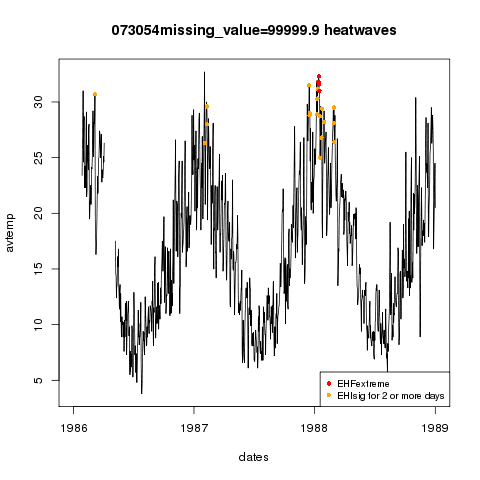
\includegraphics[width=\textwidth]{WestWyalongHeatwaves19861988.png}
\caption{WestWyalongHeatwaves19861988.png}
\label{fig:WestWyalongHeatwaves19861988.png}
\end{figure}
\clearpage

\subsection{ Discuss issues identified with the EHI indexes for further thought}

 \begin{itemize}
 \item the threshold used as the start and end of a heatwave.  the upper quintile was selected a priori but could use a calibration approach to well known heatwaves identified by news media?
 \item integration of the index thoughout the duration of the heatwave could then be more objective (John does a conditional cumulative sum for the whole heatwave, integrating EHF values when above zero, however he decides arbritrarily when to start and stop summing).
 \item The use of raw temperature difference in degrees C means that the index is not comparable between zones that are hot on average and zones that are cold on average.  Can this be normalised by using percentiles?
 \item The use of the standard 1971-2000 reference period means that well get more and more heatwaves even though we know that the population acclimatises to recent norms and it is actually deviations from that which cause health effects.
 \end{itemize}
 
 

\subsection{go}


%% \section{The end}




\end{document}
